\documentclass[tikz, border = 10pt]{standalone}

\usepackage{newpxtext,newpxmath}   % /upbeta
\usepackage{amsmath}
\renewcommand{\familydefault}{\sfdefault}
\usepackage{mathastext}

\usetikzlibrary{positioning, calc, quotes, arrows.meta}

\tikzset{
  every edge quotes/.style = {fill = white},
  manifest/.style = {draw, minimum width = 1 cm, minimum height = 0.85 cm},
  regression/.style = {-{Stealth[length = 1.5mm]}, shorten > = 1pt, inner sep = 1.5pt}
  }

\begin{document}
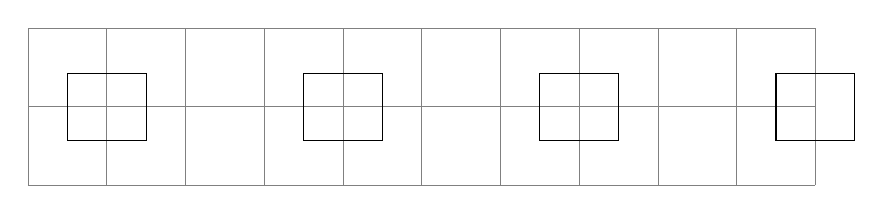
\begin{tikzpicture}

%% Manifest
\draw [help lines] (-1, -1) grid (9, 1);

\node [manifest] (x1) {};
\node [manifest] (x2) at (3, 0) {};
\node [manifest] (x3) at (6, 0) {};
\node [manifest] (x4) at (9, 0) {};

\end{tikzpicture}
\end{document}